\documentclass{article}

% Language setting
% Replace `english' with e.g. `spanish' to change the document language
\usepackage[english]{babel}
\usepackage{placeins}  % 导言区


% Set page size and margins
% Replace `letterpaper' with `a4paper' for UK/EU standard size
\usepackage[letterpaper,top=2cm,bottom=2cm,left=3cm,right=3cm,marginparwidth=1.75cm]{geometry}
\usepackage[affil-it]{authblk} % 加载 authblk 宏包

% Useful packages
\usepackage{amsmath}
\usepackage{graphicx}
\usepackage[colorlinks=true, allcolors=blue]{hyperref}

% 提及无监督的概念，
\title{Scalable representation learning in dense connectomes with hierarchical skeleton graph networks / Coordinate-free topological representation captures intrinsic neuronal identity in dense connectomes}

\author{
}

\date{
    $^1$ Institution A \\
    $^2$ Institution B \\
    $^3$ Institution C \\
}


\begin{document}
\maketitle
\begin{abstract}
Electron microscopy connectomes provide synaptic-resolution reconstructions of neuronal morphology and wiring at unprecedented scale, but converting these data into scalable and transferable neuronal representations remains a central computational challenge. Existing graph neural networks are poorly suited to contrastive learning on finely sampled skeletons because complete neuronal trees contain thousands of nodes, and conventional spatial representations are highly sensitive to non-functional morphological variation and system-specific coordinate symmetries. Here we present a representation-learning framework for dense connectomes that combines hierarchical skeleton decomposition with graph contrastive learning, enabling training on finely sampled synapse-annotated skeletons under practical memory constraints. Applied to the Drosophila FlyWire dataset, the framework supports learning on skeletons with up to 3,500 nodes and improves classification performance by up to 31\% relative to coarse structural representations. We further distinguish coordinate-aware morphology from coordinate-free topology and show that topology yields more robust clustering and few-label classification by reducing sensitivity to developmental variation, spatial position and symmetry. Across multiple neuronal populations, these results identify topology as a stable basis for neuronal identity and establish a scalable strategy for cross-scale representation learning in connectomics.


%Serial electron microscopy provides micro-connectome datasets containing massive neuronal morphologies and connectivity maps, posing analytical challenges. Automated methods such as NBLAST, which employs curve-distance algorithms, and GraphDINO, which applies contrastive learning techniques, accelerate skeleton-based neuronal analysis but cannot simultaneously achieve multimodal integration. Here, by assigning features such as diameters, synaptic targets or any local node embedding to fine skeleton nodes, comprehensive skeletons can maximize the utility of micro-connectomic data at relatively low computational cost. However, conventional graph neural networks remain insufficient for contrastive learning on fine skeletons with large numbers of nodes, a limitation we address using subgraph decomposition combined with a tailored hierarchical graph neural network architecture (HGNNA). We apply contrastive learning to the FlyWire dataset using simplified skeletons with 200 nodes and comprehensive skeletons with 3500 nodes, and testing on Kenyon Cell (KC) classification shows that the richer neuronal information in comprehensive skeletons can be captured by graph neural network to improve prediction accuracy. Subsequently, in the absence of cell type labels, the morphology embeddings of KC neurons and their axonal segments independently show that Hemilineage and cell types are significantly separated under t-SNE dimensionality reduction. Thereafter, the testing results on the FlyWire optic lobe and MICrONS datasets are less straightforward, and the article discusses the relationship between contrastive learning, morphology, and absolute coordinates in terms of input, suggesting that appropriate input features and data augmentation strategies should be adopted across different species or brain regions. Finally, we reassign the learned morphological representations of neurons in FlyWire as embedding vectors to their associated synaptic nodes. The article thus discusses the compatibility of the method with embedding vectors and the potential extension to connectivity analysis.
\end{abstract}

\section{Introduction}
% 【电镜数据——发展需求】 % *背景和重要性
Understanding neural computation requires compact, informative representations of neuronal structure and wiring. Recent advances in serial-section electron microscopy have produced dense connectomes with synaptic-resolution reconstructions for up to hundreds of thousands of neurons, including the Drosophila hemibrain, FlyWire, and MICrONS datasets. These resources provide an unprecedented opportunity to study neuronal identity, circuit organization and structure–function relationships at scale, but they also create a fundamental computational challenge: how to convert richly detailed neuronal reconstructions into compact, informative and transferable representations that support both cell-level and circuit-level analysis.

Traditional connectomic analysis has relied heavily on hand-crafted features derived from morphology, connectivity or both. Although such approaches can be effective in well-studied systems, they are difficult to scale and often require substantial expert intervention. This is particularly limiting in newly reconstructed datasets, where the relevant features are not known in advance and manual annotation remains expensive. A more general solution is to learn neuronal representations directly from the data, so that neurons with similar structural identity cluster together without extensive feature engineering.

Recent work has begun to apply representation learning and graph neural networks (GNNs) to connectomic data. However, existing methods face two major limitations. First, they typically operate on simplified skeletons or heavily aggregated graph descriptions, thereby discarding fine structural information and weakening the link between morphology and synaptic organization. Second, they often treat absolute spatial coordinates as primary inputs, making the learned representation sensitive to coordinate-specific effects that may not reflect neuronal identity itself.

These limitations matter because many biologically informative distinctions are expressed at fine structural scales. Synapse placement, local branching structure, and the relationship between neuronal arbors and their inputs are not adequately captured by coarse skeletons. Ideally, representation learning would operate directly on high-resolution skeletons enriched with synaptic annotations. In practice, however, this is computationally difficult: complete neuronal skeletons can contain thousands of nodes, making direct graph learning memory-intensive and poorly suited to large-scale contrastive learning.

% 【电镜数据——数据形式、现有研究——形态、连接】*现有研究的局限性 *研究趋势 *在新趋势下的关键问题
%Historically, neuronal analysis relied on manually defined statistical features. Although supervised deep learning and unsupervised clustering improved accuracy and efficiency, they remain constrained by a reliance on hand-crafted descriptors and expert validation, which limits scalability and introduces bias. In practice, neuronal types in previously unexplored neural systems are typically inferred by comparing and summarizing morphological and connectivity patterns across large populations of neurons. Even when it is known which features are informative for neuronal classification, extracting and validating these features requires extensive and careful analysis by domain experts. Hence, our work is motivated by a fundamental premise: if our understanding of a target neural system is extremely limited—analogous to the perspective of a non-expert numerical analyst—can meaningful organizational principles still be discovered directly from the data, enabling the identification of similar neuronal types and the discrimination of distinct ones? To mitigate these issues, unsupervised representation learning has been introduced into this area, utilizing contrastive learning and Graph Neural Networks (GNN) to analyze connectome data from a uniformly modified initial form. These approaches typically treat morphology as skeletons or connectivity as connectivity graph separately. Crucially, however, insights from circuit discovery indicate that neither feature is sufficient in isolation; rather, the specific connectivity along neuron neurites is essential for precise neuronal identification.

To address this problem, we introduce a framework that combines hierarchical skeleton decomposition with graph contrastive learning. The core idea is to decompose each finely sampled neuronal tree into smaller subgraphs, encode them hierarchically, and progressively integrate local and global structure. This yields a scalable graph-learning framework that preserves synapse-aware structural detail while substantially reducing memory cost.

% 【神经元的精细建模】 *我们的解决方案，精细骨架及挑战* 不提融合图谱的概念，而是从单细胞视角加入连接性这一概念。To enrich the neuritic skeleton是为了实现对应的表示学习
%To enrich the neuritic skeleton with both structural and connection-specific attributes, a proper initial form of finely sampled skeletons with extra node feature is proposed. A high-resolution resampling of the neuritic tree that increases node density enables precise mapping of individual synapses onto the underlying morphology. However, this dense representation substantially increases the computational burden, making large-scale graph learning prohibitively expensive. % 【子图分解和分级图神经网络框架】 *我们的解决方案子图分解和HGNNA
%To overcome this limitation, we introduce a skeleton decomposition strategy in conjunction with a hierarchical graph neural network architecture (HGNNA). This approach reduces the computational cost by more than an order of magnitude, enabling representation learning for hundreds of thousands of neurons with fine structure and connectivity under practical resource constraints.

Using this framework we also reveal a broader representational issue. Neurons are embedded in anatomical coordinate systems with different symmetry structures across brain regions and species. Some populations exhibit mirror symmetry, others approximate translational symmetry, and still others are arranged on curved surfaces. When absolute coordinates are used as input features, neurons of the same type may receive different representations because of developmental variation, hemispheric placement or positional symmetry rather than true differences in structural identity. This motivates a distinction between two representation regimes: coordinate-aware morphology, which includes explicit spatial coordinates, and coordinate-free topology, which removes coordinates while preserving graph structure and node-level annotations.

% 【空间对称性在不同系统中存在差异】 *问题：坐标
%During our investigation, we found that neuronal coordinate systems exhibit distinct symmetry properties across biological systems. For instance, cortical neurons of the same type often display translational symmetry, whereas typical neurons in Drosophila instead follow mirror symmetry. Within the fly optic lobe, yet another pattern emerges: neurons exhibit symmetry consistent with movement along a curved surface. These heterogeneous coordinate symmetries impose inherent constraints on methods that explicitly rely on spatial positions. In contrast, when spatial coordinates are excluded, the topological organization of neuronal skeletons may remain largely consistent across neurons of similar types, irrespective of the symmetry of their underlying coordinate systems.

Here we present a scalable representation-learning framework for dense connectomes that combines hierarchical skeleton decomposition with graph contrastive learning. Using FlyWire as the primary testbed, with Kenyon cells as a central benchmark and additional analyses in optic-lobe and broader FlyWire populations, we show that fine skeletons substantially improve classification, that coordinate-aware morphology is sensitive to developmental and geometric confounds, and that coordinate-free topology yields more robust clustering and few-label inference. Together, these results define a scalable strategy for cross-scale representation learning in connectomics and identify topology as a stable representation layer for neuronal identity.

% 【形态、拓扑、连接】 *具体研究的路线
%Motivated by this observation, we construct skeletons with coordinates as morphological representations and skeletons without coordinates as topological representations. Connectivity information is further incorporated by enriching each skeleton node with synaptic annotations and target embeddings. This joint formulation enables a unified analysis of both neuronal morphology and connectivity at the level of individual cells.
% 【FlyWire和MICrONS】 *具体研究应用的点
%The validity and generality of the proposed representations are assessed using the FlyWire and MICrONS datasets. For the FlyWire dataset, we adopt the classification of Kenyon cell (KC) neuron populations as the main benchmark to assess the representation capability.
% 为了将大型骨架的图神经网络学习我们从拓扑和连接两个角度【大型骨架和模型】【拓扑结构】【拓扑连接性】【应用】 

% **精细采样骨架的无监督学习为分类任务捕获更多信息**
\section{Hierarchical graph learning enables representation learning from finely sampled skeletons}

%{Unsupervised Learning on Finely Sampled Skeletons Captures Richer Information for Classification Tasks} % 更多的描述放在method中
% 【骨架节点数统计】

A basic challenge in dense connectomics is choosing a structural resolution that preserves biologically meaningful detail without becoming computationally intractable. To address this, we analyzed FlyWire skeletons together with their synaptic annotations. Each synapse was mapped to its nearest skeleton node, and nodes were labeled as presynaptic, postsynaptic, branch or terminal nodes where appropriate ({Fig.\ref{fig:morph_classify}a}). We refer to these as meaningful nodes, because they anchor both local morphology and synaptic context.

The distribution of meaningful node counts across all skeletons are shown in {Fig.\ref{fig:morph_classify}b}. Across FlyWire, most neurons contained fewer than 1,000 meaningful nodes, whereas a substantial subset contained several thousand. Based on the cumulative distribution of meaningful node counts, we selected 3,500 nodes as a practical upper bound, covering 96.37\% of neurons in the dataset ({Fig.\ref{fig:morph_classify}c}). Skeletons exceeding this threshold were randomly downsampled. This preserves substantially more structural information than coarse skeletonization while keeping graph size manageable.

%To address the question of how many nodes are sufficient for the description of a neuron skeleton, we selected a publicly available dataset: FlyWire (adult Drosophila) for statistical analysis. FlyWire provides finely sampled skeletons and detailed synaptic information. For each synapse, we assigned it to the nearest node of the corresponding skeleton and labeled the nodes as either 'pre-synapse,' 'post-synapse,' or 'fork node,' and 'end node' where appropriate (a demonstration is shown in {Fig.\ref{fig:morph_classify}a}). A node is considered a "meaningful node" if it is labeled as one of these four types. We then counted the number of meaningful nodes for each skeleton in the dataset. The distribution of meaningful node counts across all skeletons is shown in {Fig.\ref{fig:morph_classify}b}. Most skeletons contain fewer than 1,000 meaningful nodes, while a small fraction possess several thousand nodes. Based on the cumulative percentage calculation ({Fig.\ref{fig:morph_classify}c}) for the distribution of meaningful nodes, we set the threshold at 3,500 nodes in our application, which covers 96.37\% of cells in FlyWire. Skeletons with more than 3500 nodes will have nodes randomly dropped to maintain a skeleton with 3500 nodes.

% Figure 1. 骨架节点数统计 # MICrONS可以放在extended
\begin{figure}[htbp]
\centering
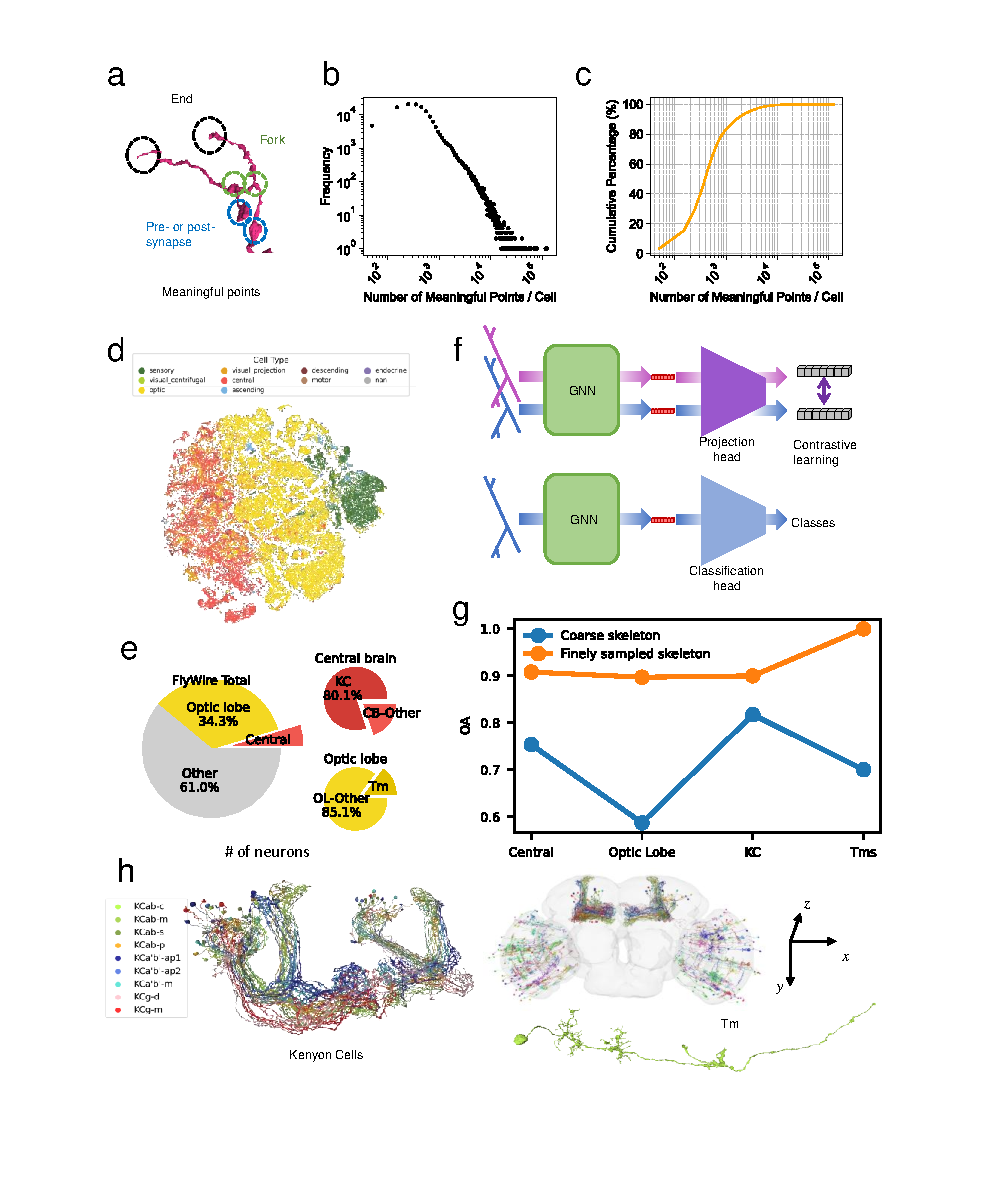
\includegraphics[width=1\linewidth]{figures/Fig1_0202.pdf}
\caption{(a) Example of a neuron with end, fork, pre- or post-synapse label. (b) Distribution of meaningful node counts across all neuron skeletons in FlyWire. (c) Cumulative percentage of neuron skeletons as a function of meaningful node counts. (d) t-SNE visualization of morphology representations colored by super classes for all neurons in FlyWire. (e) Pie graph of the target neurons groups of four tasks. (f) Schematic of cell-type classification after contrastive learning of morphology representations. (g) Classification accuracy comparison between coarse and finely sampled skeletons across four tasks: Central Brain (CB), Optic Lobe (OL), Kenyon Cells (KC), and Transmedullary neurons (Tm). (h) Example morphologies of KC and Tm neurons.}
\label{fig:morph_classify}
\end{figure} 

% 3500 进行 单层8 节点子图分解，邻接矩阵大小将会变为原来的1.8%。
% 【测试的方法和对象】
To process skeletons at this scale, we developed a skeleton decomposition strategy together with a hierarchical graph neural network architecture (HGNNA). Rather than applying a single GNN to a graph containing thousands of nodes, the framework partitions each neuronal tree into smaller subgraphs and processes them hierarchically. Local structure is encoded first, and these local embeddings are then recursively integrated into higher-level representations. This makes graph contrastive learning on fine, synapse-aware skeletons computationally feasible.
%To make learning feasible at this resolution, we implemented hierarchical skeleton decomposition together with a hierarchical graph neural network architecture (HGNNA). The model applies graph contrastive learning to decomposed subgraphs and aggregates information across scales, enabling high-resolution skeletons to be processed under practical memory constraints. This design allows the latent space to capture structural information that is inaccessible to coarsely sampled skeletons while preserving scalability at connectome scale.

The computational gain can be seen directly in adjacency storage. For a graph with $N$ nodes decomposed into subgraphs of size $n$, adjacency-memory cost is reduced from $N^2$ to approximately $Nn + \frac{N^2}{n^2}$. For $N = 3500$ and $n = 19$, this corresponds to an approximately 122-fold reduction in adjacency-related memory cost. In practice, efficiency also depends on the number of hierarchical levels and the architecture used at each level, but the key result is simple: hierarchical decomposition resolves the memory bottleneck that otherwise prevents contrastive learning on finely sampled neuronal skeletons.

The trained encoder maps each input skeleton to a latent embedding without using cell-type labels during pretraining. When coordinates are included among node features, the resulting embedding is treated as a morphology representation. When coordinates are excluded, it is treated as a topology representation. These two regimes form the basis for the analyses below.

\section{Fine skeletons carry substantially richer information than coarse representations}

We next asked whether the additional information preserved in fine skeletons improves downstream neuronal classification. After contrastive pretraining, the projection head was replaced with a classification head (Fig. 1f) and evaluated on four FlyWire tasks: central brain (CB), optic lobe (OL), Kenyon cells (KC), and transmedullary neurons (Tm). These tasks span both broad neuronal populations and more specific subtype distinctions. CB and OL together constitute 38.9\% of all neurons in FlyWire and represent broad central and peripheral neuronal populations, respectively (Fig. 1e). KC and Tm are more specific neuronal classes within CB and OL, and can each be subdivided into finer types, with representative morphologies and spatial distributions shown in Fig. 1h and Fig. 2g.

%To verify whether the enhanced expressiveness of comprehensive skeletons can be effectively utilized by our designed HGNNA, we conducted cell-type classification tasks on the FlyWire dataset. Following the morphology representation learning stage, the projection head was replaced with a classification head for supervised evaluation ({Fig.\ref{fig:morph_classify}f}). The test is performed on the classification of types in central brain (CB), optic lobe (OL), Kenyon cells (KC), and transmedullary neurons (Tm) types. Among these, CB and OL constitute a large proportion (38.9 percent) of all neurons in FlyWire, representing central and peripheral neural populations, respectively; we performed cell-type classification tests on these two populations. KC and Tm are neuronal classes in CB and OL, respectively, and can be further subdivided into more detailed types, with neuronal morphologies and distributions shown in {Fig.\ref{fig:morph_classify}h} and {Fig.\ref{fig:morph_sensitivity}g}. 


% 【测试的结果】不是都采用缩写是为了提高可读性。KC和Tm采用了缩写。
Finely sampled skeletons consistently outperformed coarse skeletons across all four tasks. Accuracy increased from 75.38\% to 90.81\% in CB, from 58.72\% to 89.71\% in OL, from 81.74\% to 90.00\% in KC, and from 70.03\% to 100.00\% in Tm. These significant gains show that fine structural sampling is not a cosmetic refinement. It provides substantially richer signal for representation learning across multiple neuronal systems.

The Tm result is especially notable. With fine skeletons, morphology-based representation learning achieved perfect classification. This suggests that, at least in this setting, sufficiently detailed morphology can fully resolve subtype identity without explicit connectivity features. More broadly, it indicates that an important limitation of earlier graph-based approaches may lie not only in model design, but also in the structural simplification imposed at the input stage.

These findings establish the first main conclusion of the study: high-resolution skeletons contain substantially more useful signal for neuronal representation learning than coarse skeletons, and a scalable framework is therefore required to exploit that signal.

%The classification accuracy results are summarized in {Fig.~\ref{fig:morph_classify}g}. Across all four classification tasks, finely sampled skeletons consistently outperform coarse skeletons. Specifically, the accuracy improvements are: Central brain classification improves from 75.38\% to 90.81\% (15.43\% gain), optic lobe classification from 58.72\% to 89.71\% (30.99\% gain), KC classification from 81.74\% to 90.00\% (8.26\% gain), and Tm classification from 70.03\% to 100.00\% (29.97\% gain). Notably, while the visual system neurons (in the tasks of OL and Tm) demonstrate notably larger accuracy gains compared to central brain populations, this pronounced improvement in visual system classification suggests that neuronal types in the optic lobe are more tightly coupled with their morphological features. The exceptional performance on Tm neurons (100\% accuracy with finely sampled skeletons) indicates that morphology representation alone can completely distinguish Tm types, contrary to previous studies suggesting that some Tm types require connectivity information for proper classification. This demonstrates that the detailed morphological information captured by fine-grained skeleton representations is particularly effective for distinguishing visually-specialized neuronal types.


% **形态对非功能性特征、空间位置和对称性敏感**
\section{Morphology representation is confounded by developmental and geometric variation} 
% 主要转折
% 用KC说明影响因素：发育谱系、对称性，神经元之间的空间竞争。
% 说明形态表示的局限性。
% 现在的图内容还可以，这个后续再优化，先放下不动。
% 形态-Tm的结果放在这里一部分。从这一点出发，我们将FlyWire神经元骨架经过GNN后输出的latent表示进行t-SNE降维。为了观察不同类别神经元的latent分布情况，将不同类型神经元用不同颜色表示（图1d 所有FlyWire神经元不同super class的分布情况，图2a 所有KC神经元不同类型的分布情况，图2h Tm不同类型的分布情况）。

Contrastive learning derives features without cell-type labels, raising the question of whether the learned latent space can itself reveal meaningful neuronal organization. To address this, We therefore examined whether morphology representations could recover meaningful neuronal organization without supervision. At the scale of the full FlyWire dataset, the latent space separated major neuronal superclasses, indicating that the representation captures broad structural organization. At finer scales, however, the latent geometry also reflects additional forms of biological and geometric variation. 

%It is worth noting that contrastive learning is an unsupervised method for deriving features from large datasets. Thus, under the assumption of having no cell type labels, one may ask whether the latent representations can be exploited to analyze the commonalities and differences among neurons. Starting from this perspective, we performed t-SNE dimensionality reduction on the latent representations output by the GNN for FlyWire neuron skeletons. To visualize the latent distribution of different neuronal categories, neurons of different types were represented using different colors ({Fig.~\ref{fig:morph_classify}d} shows the distribution of different super classes across all FlyWire neurons, {Fig.~\ref{fig:morph_sensitivity}a} shows the distribution of different types among all KC neurons, and {Fig.~\ref{fig:morph_sensitivity}h} shows the distribution of different Tm types).

% Figure 2. 
\begin{figure}[htbp]
\centering
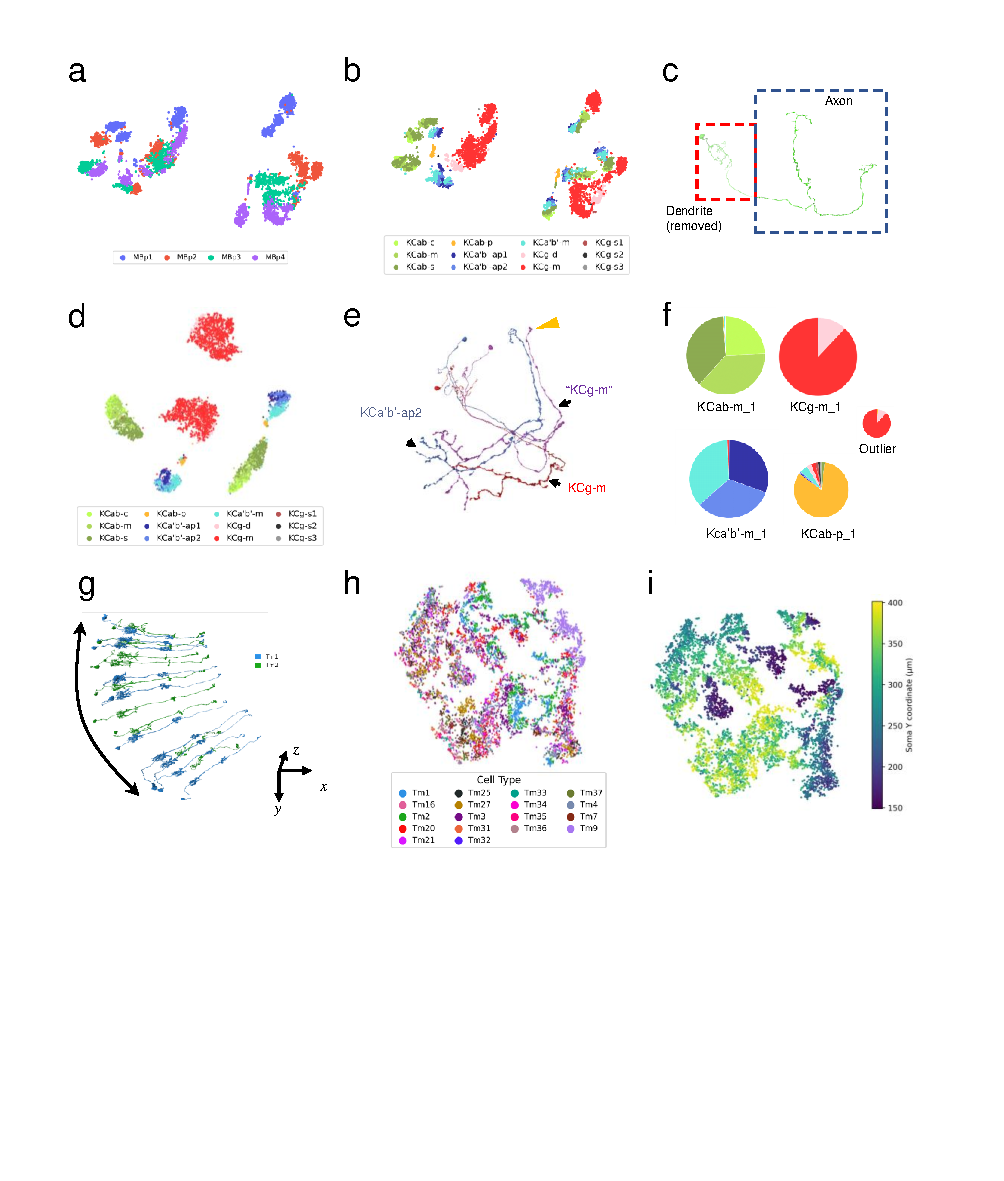
\includegraphics[width=1\linewidth]{figures/Fig2_0202.pdf}
\caption{(a) and (b) t-SNE visualization of morphology representations of Kenyon Cells (KCs). (c) Morphological differences in dendritic segments among KC hemilineages. (d) t-SNE visualization of morphology representations of KCs after removing dendritic segments. (e) Example of a misclassified KC neuron. (f) Pie chart showing the correspondence between clustering types and original label types. (g) Morphological differences in Tm neurons along the y-coordinate. (h) t-SNE visualization of morphology representations of Tm neurons. (i) Correlation between the y-coordinate of the soma and the latent representation of Tm neurons.}
\label{fig:morph_sensitivity}
\end{figure}

% 错误类型标签存在于calssificaiton.csv中，网页上直接查询是正常的。
This is particularly clear in Kenyon cells. KC morphology embeddings form distinct clusters (Fig. 2b), but these clusters reflect not only KC subtype, but also developmental hemilineage and hemisphere. Thus, the latent space captures biologically real structure, but not structure aligned solely with neuronal type. This is a critical point: morphology representations can be information-rich while still being poorly matched to the goal of recovering a coordinate-invariant notion of neuronal identity.

The source of this effect becomes clearer when KC anatomy is examined directly. KC neurons differ systematically in their dendritic segments across hemilineages (Fig. 2c), and these differences are largely independent of the canonical KC subtype labels (ref.X). To isolate this contribution, we removed dendritic segments from the network input without retraining the model (Fig. 2d). Under this manipulation, hemilineage-driven separation was reduced and the latent space aligned more closely with hemisphere and KC subtype. The resulting five-type clustering more closely matched the expected KC organization (consistency reaches X\%). This shows that morphology representations are strongly influenced by developmental structure that is meaningful in its own right, but orthogonal to the classification objective.

The KC latent space also exposed likely annotation errors. Neurons whose labels were inconsistent with their local embedding neighborhoods could be identified as probable misannotations. One example is shown in Fig. 2e, where a KCa'b' neuron was incorrectly classified as KCg-m in the original type labels. This highlights an additional use of the learned representation: beyond prediction, it can help identify inconsistencies in existing labels and improve dataset curation.

%The distribution of KC types exhibits multiple clusters ({Fig.~\ref{fig:morph_sensitivity}b}). Multiple clusters correspond to KC cell types, different hemilineages and left-right brain hemispheres. KC neurons display pronounced morphological differences in their dendritic segments due to distinct developmental lineages ({Fig.~\ref{fig:morph_sensitivity}c}), and these differences are independent of KC classification types (ref.X). By removing dendritic segments from the network input without retraining, we can eliminate the effects of developmental lineage ({Fig.~\ref{fig:morph_sensitivity}d}), revealing only left-right hemispheric and KC cell type differences. Clustering the morphological representations without dendritic segments yields the primary classification clusters within KC types; under this five-type clustering scheme, consistency reaches X\% (the correspondence between clustering types and original label types is shown in the pie chart in {Fig.~\ref{fig:morph_sensitivity}f}). Furthermore, by examining neurons of other types that fall within single-type clusters in {Fig.~\ref{fig:morph_sensitivity}d}, we identified instances of mislabeling. {Fig.~\ref{fig:morph_sensitivity}e} shows a KCa'b' neuron that was incorrectly classified as KCg-m in the type labels.

% !补充Tms中的latent与y坐标关联性
A related limitation appears in optic-lobe populations. In Tm neurons, morphology representations achieve excellent supervised classification, yet the unsupervised latent space remains fragmented, with a Silhouette score of only 0.008 (Fig. 2h). This apparent contradiction reflects geometric confounding rather than lack of signal. Optic-lobe neurons are arranged along a curved surface, and Optic-lobe neurons are arranged along a curved surface, and this fragmentation is partly attributable to the rotational and translational symmetries inherent to optic lobe neurons, as well as to non-functional segments generated during development. Consistent with this interpretation, we found a significant association between soma position and latent structure along the y axis (Fig. 2i). As a result, neurons of the same type but at different positions can receive distinct morphology representations, weakening unsupervised clustering despite strong discriminative signal.
%The t-SNE visualization of Tm neurons reveals a more dispersed distribution, with Silhouette score of 0.008. This fragmentation is partially attributable to the rotational and translational symmetries exhibited by optic lobe neurons, as well as the presence of non-functional segments arising from developmental processes. By computing the correlation between the y-coordinate of the soma and the latent representation of the cell, a significant association emerges, as visualized in {Fig.~\ref{fig:morph_sensitivity}i}. 

Taken together, these results show that coordinate-aware morphology is sensitive to developmental variation, absolute position, and system-specific coordinate symmetry. These factors may themselves be biologically meaningful, but they can also dominate the latent space in ways that obscure neuronal identity. This motivates a coordinate-free alternative.
%These findings indicate that non-functional segments arising from development and the spatial symmetry of neurons significantly impact morphological representations, posing challenges for unsupervised clustering.

% **拓扑表示在聚类方面的优势**
\section{Coordinate-free topology yields more robust neuronal representations} 

To disentangle structural identity from coordinate-dependent variation, we constructed a representation that preserves skeletal connectivity and node-level annotations while removing explicit spatial coordinates. We refer to this representation as topology (Fig. 3a). In this regime, branching structure, graph organization, and synapse-related node information are retained, but absolute geometry is excluded.
%A portion of the sensitivity of morphological representations arises from their dependence on spatial coordinates. To disentangle this effect, we removed coordinate inputs while retaining the skeletal topological structure, which we refer to as the topological representation (Fig.\ref{fig:topology}a). Compared with the morphological representation, the topological representation exhibits consistently improved intra-class compactness and inter-class separability across multiple evaluation settings, including all-neuron super classes, optic-lobe classes, Tm classes, and KC classes (Fig.\ref{fig:topology}b–e, g–i). 

% 四个任务具体的数值
Across multiple FlyWire populations, topology embeddings yielded more coherent class structure than morphology embeddings. In Kenyon cells, representing a 1.49-fold improvement in class separation, while the average intra-class distance decreases from 4.900 to 3.721, indicating 24.1\% tighter within-class clustering. The corresponding Silhouette score improved from -0.048 to 0.090. For Tm neurons, the inter-class distance increases from 12.077 to 12.692 (1.05-fold), while intra-class distance decreases from 9.445 to 6.696 (29.1\% reduction), with Silhouette scores of 0.008 and 0.210 respectively. Similar improvements are observed for neurons in CB (Silhouette scores: -0.019 vs 0.066) and OL (Silhouette scores: -0.149 vs 0.059). These results indicate that removing coordinates (Fig. 3e) suppresses nuisance variation while preserving type-related organization (Fig. 2d).
%Specifically, for KC neurons, the average inter-class distance increases from 5.639 (morphology) to 8.382 (topology), representing a 1.49-fold improvement in class separation, while the average intra-class distance decreases from 4.900 to 3.721, indicating 24.1\% tighter within-class clustering. The Silhouette score improves from -0.048 (morphology) to 0.090 (topology). For Tm neurons, the inter-class distance increases from 12.077 to 12.692 (1.05-fold), while intra-class distance decreases from 9.445 to 6.696 (29.1\% reduction), with Silhouette scores of 0.008 and 0.210 respectively. Similar improvements are observed for neurons in CB (Silhouette scores: -0.019 vs 0.066) and OL (Silhouette scores: -0.149 vs 0.059). Together, these quantitative metrics demonstrate that the topological representation (Fig. \ref{fig:topology}e) provides clear advantages over the morphological representation (Fig.Fig.~\ref{fig:morph_sensitivity}d) in unsupervised clustering.

% 小比例的OL Tm CB重新测试小训练集分类
% These advantages are further reflected in few-label classification performance. We conducted classification experiments using only a small fraction of labeled data, selecting limited proportions of labels for CB, OL, KC, and Tm classification tasks. As shown in Fig. \ref{fig:topology}f, the topological representation consistently outperforms the morphological representation across all four tasks, achieving accuracy improvements of X1%, X2%, X3%, and X4%, respectively.

The same advantage appears in low-label settings. In five-class KC classification, reducing the fraction of labelled data from 80\% to 10\% caused morphology-based performance to drop from 98\% to 85\%, whereas topology-based performance remained stable at 89\%. Comparable trends were observed in OL and CB tasks. By contrast, the accuracy of topology-based classification remains nearly unchanged and exceeds that of morphology-based classification at 10\% labeling. Thus, topology is not just a cleaner visualization space; it is a more label-efficient and transferable representation of neuronal identity.

%These advantages are further reflected in few-label classification performance. We conducted classification experiments using only a small fraction of labeled data, selecting limited proportions of labels for CB, OL, KC, and Tm classification tasks. As shown in Fig. \ref{fig:topology}f, in the five-class Kenyon cell classification task, reducing the labeled data ratio from 80\% to 10\% leads to a pronounced performance degradation in morphology-based representations (from 98\% to 85\%). By contrast, the accuracy of topology-based classification remains nearly unchanged and exceeds that of morphology-based classification at 10\% labeling, highlighting its improved robustness.

This contrast between morphology and topology is the central conceptual result of the paper. Including coordinates may increase descriptive richness, but it also increases sensitivity to developmental and geometric confounds. By contrast, coordinate-free topology provides a more stable intermediate representation for clustering and few-label inference. This does not imply that coordinates are unimportant. Rather, it suggests that in scalable connectomic representation learning, geometry and identity should be treated as related but partially separable layers of description.

% Figure 3. 形态聚类尝试与局限性,KC Tm
\begin{figure}[htbp]
\centering
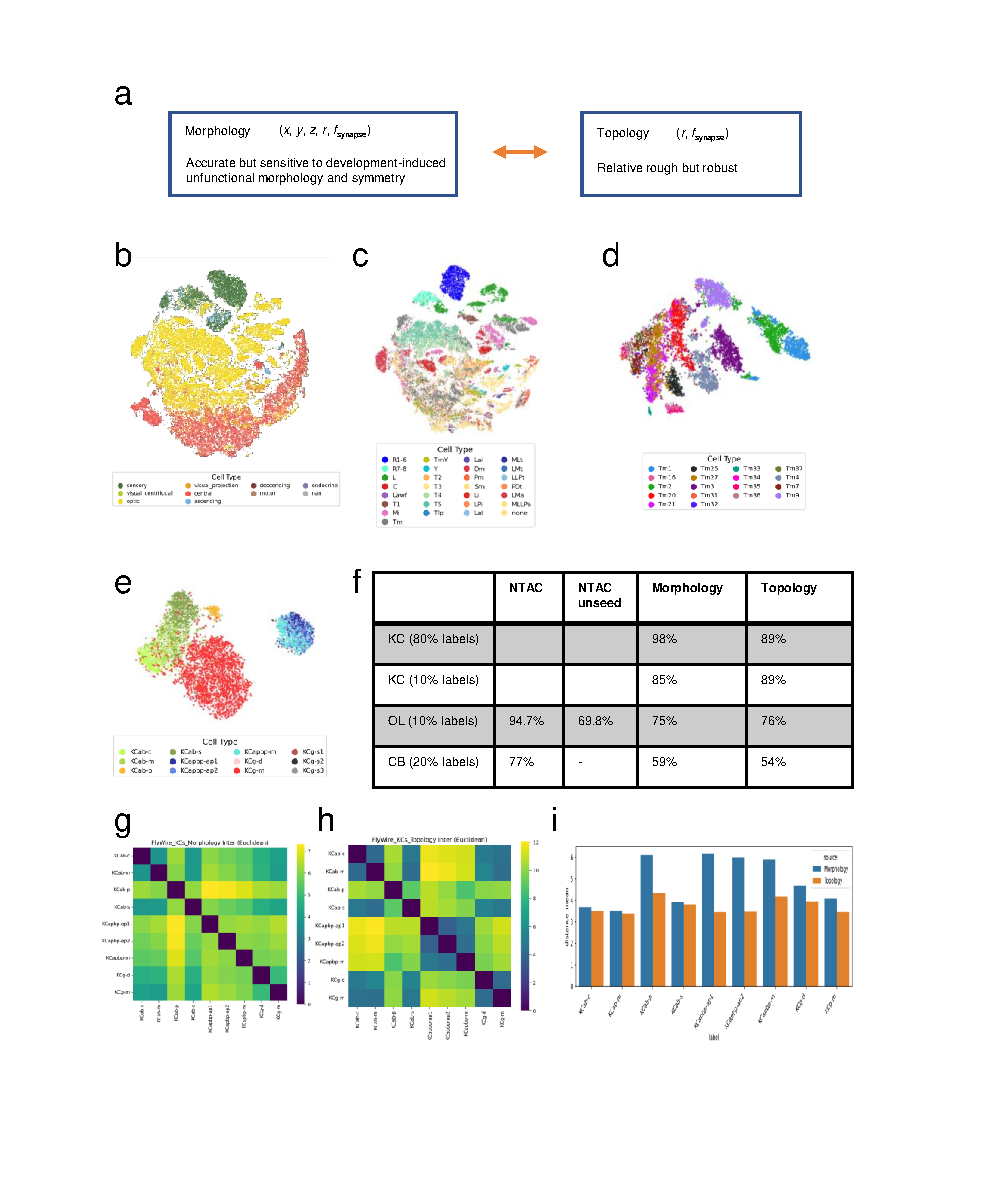
\includegraphics[width=1\linewidth]{figures/Fig3_0202.pdf}
\caption{(a) Schematic of topology representation without coordinate inputs. (b–e) t-SNE visualizations of topological representations colored by super classes for all neurons, classes within the optic lobe, Tm classes, and KC classes, respectively. (f) Few-label classification accuracy comparison between topology and morphology representations across four tasks. (g–i) Quantitative metrics of intra-class and inter-class distances for topology representations in all neurons, optic lobe neurons, and Tm neurons, respectively.}
\label{fig:topology}
\end{figure} 

\section{Broader implications across systems and for downstream connectomic analysis} 

The clearest findings in this study come from FlyWire, particularly the KC and Tm benchmarks. However, the broader lesson is not restricted to these populations. Additional experiments in the FlyWire optic lobe and observations in MICrONS suggest that the interaction between morphology, topology, contrastive learning, and coordinate symmetry is system-dependent. In some settings, results are less straightforward, likely because different neural systems obey different geometric symmetries and therefore require different feature designs or augmentation strategies. This is not merely a technical nuisance; it is an empirical property of connectomic representation learning. The geometry of the biological coordinate system directly shapes the behavior of learned representations.

The framework also has a natural path toward connectivity analysis. Once a neuron-level embedding has been learned, that embedding can be reassigned to its associated synaptic nodes, providing a bridge between cell-level representation learning and future graph- or circuit-level models. Although such downstream analyses are beyond the scope of the present work, the learned representations produced here are explicitly compatible with that extension


\FloatBarrier

\section{Discussion}

We developed a scalable framework for representation learning in dense connectomes by combining hierarchical skeleton decomposition with graph contrastive learning. The framework addresses a central computational bottleneck in connectomics: how to learn from richly annotated, finely sampled neuronal skeletons without incurring prohibitive memory cost. By decomposing tree-like neuronal graphs into subgraphs and processing them hierarchically, HGNNA enables contrastive learning on high-resolution skeletons containing thousands of nodes and preserves synapse-aware structural detail that is inaccessible to coarse representations.

The first major conclusion is practical. Fine skeletons substantially improve downstream classification across multiple neuronal populations. These gains show that high-resolution structural input is not merely a cosmetic improvement over coarse skeletonization. In some systems, especially those with highly specialized morphologies, that additional detail is strongly predictive of neuronal identity. This suggests that a major limitation of previous graph-based approaches may not lie only in model design, but also in the degree of structural simplification imposed at the input stage.

The second major conclusion is conceptual. Coordinate-aware morphology embeddings are sensitive to developmental variation, absolute position and coordinate symmetry. These sources of variation can be biologically meaningful, but they can also interfere with the recovery of neuronal identity in unsupervised or low-label settings. This is particularly evident in KCs, where morphology reflects lineage as well as type, and in Tm neurons, where positional symmetry in the optic lobe distorts latent geometry. Coordinate-free topology mitigates these effects by focusing on branching structure and local graph organization rather than absolute placement in space.

This distinction between morphology and topology points to a broader principle for connectomic representation learning. Richer representations are not always more robust representations. In some cases, the inclusion of absolute geometric information increases descriptive fidelity while reducing transferability across neurons or systems. By contrast, topology can act as an intermediate representation layer that is less sensitive to system-specific coordinate symmetries and therefore more stable for clustering, few-label inference and potentially downstream integration with connectivity features.

At the same time, the work highlights several boundaries and open questions. First, topology is not universally sufficient for all tasks. Some biological questions depend explicitly on geometry, location or symmetry, and coordinate-aware representations may remain essential in those cases. Second, the behavior of the framework across FlyWire and MICrONS suggests that augmentation strategies and feature choices may need to be tuned to the structure of the target system rather than assumed to generalize automatically. Third, the present study primarily addresses neuron-level representation learning. Future work should test how these embeddings can best be fused with connectivity information in circuit-level models.

More broadly, our results suggest that scalable connectomic analysis should separate at least two related but distinct goals: representing neurons with sufficient descriptive richness, and learning latent spaces that preserve neuronal identity robustly across developmental and geometric variation. Hierarchical graph learning provides a practical route to the first goal, whereas coordinate-free topology provides a principled route to the second. Together, they offer a computational strategy for cross-scale representation learning in dense connectomes.


\section{Method}

\subsection{Datasets}

The primary dataset analyzed in this study was FlyWire, which provides finely sampled neuronal skeletons and synaptic annotations for the adult Drosophila brain. Additional observations were made using MICrONS to examine the broader applicability of the framework across datasets with different geometric organization. FlyWire served as the main benchmark throughout, with Kenyon cells used as the central test case for detailed analysis. Broader FlyWire populations, including central brain neurons, optic-lobe neurons, and transmedullary neurons, were also used for classification and clustering analyses.

\subsection{Synapse-aware fine skeleton construction}

\subsection{Hierarchical skeleton decomposition}

\subsection{Hierarchical graph neural network architecture}

\subsection{Memory-cost analysis}

\subsection{Contrastive learning}

\subsection{Data augmentation}

\subsection{Morphology and topology representations}

\subsection{Downstream classification and latent-space analysis}

\subsection{Embedding and connectivity analysis}

To replace below:
\subsection{Method: Graph decomposition and hierarchical graph neural network}
% Graph
% Graph decomposition history
% My graph decompositon
% 大型图处理方法有哪些
A graph can be expressed as nodes and edges, and in graph neural network operations, it is commonly represented by feature and adjacency matrices. The complete skeleton of a neuron can contain thousands of nodes to describe its intricate structure, resulting in an adjacency matrix that is particularly large and challenging to process. % Therefore, several methods have been developed, including Sampling Methods (GraphSAGE, PinSAGE), which randomly sample a subset of neighboring nodes to reduce computational complexity; Graph Partitioning (Cluster-GCN), which divides large graphs into multiple subgraphs with nodes feature clustering and executes message passing only within these subgraphs during training; and Graph Pooling (DIFFPOOL), which uses a hierarchical approach that is challenging to train, requiring each level to be trained individually before clustering and inputting to the next level. These methods are primarily applied to complex graphs, such as those formed by social networks, while the skeleton of a single neuron is typically represented as a tree (an acyclic undirected graph) in graph theory, with branches extending from the soma. Therefore, in our work, the method of graph decomposition along with hierarchical graph neural network has been proposed for the efficient processing of neuron skeletons. Our plan has the natural ability of multi-scale feature perception to contain the localized synaptic distribution and global morphology.

% 编辑1
A soma-initiated breadth-first search is performed to partition a tree-like graph into subgraphs, each containing a fixed number of \(n\) nodes. Once a subgraph reaches \(n\) nodes or has no unvisited neighboring nodes, it is finalized. A new unvisited node is then randomly selected as the seed to initiate the next subgraph. The process is visualized in \textbf{Fig}. The decomposition process can be applied multiple times to reduce the adjacency matrix. However, excessive decomposition may lead to fragmentation and increased computational overhead during the decomposition process. In our work, skeletons are decomposed twice to achieve an acceptable memory cost. The adjacency matrix of each subgraph is preserved, and inter-subgraph adjacency matrices are constructed to represent connectivity between subgraphs. A connection between two subgraphs is defined as the existence of at least one edge linking a node in one subgraph to a node in the other.

To facilitate the processing of decomposed subgraphs, a hierarchical graph neural network (HGNN) is designed to extract information from subgraphs without requiring multiple training iterations. Subgraphs with the same number of nodes are batched and processed by a graph neural network (GNN) module, which outputs latent representations for each subgraph. These latent representations along with the inter-subgraph adjacency matrices can be understand as compressed graph of the original graph, and are then processed by another module with the same design to generate a latent representation for a larger subgraph (at a middle layer) or the entire graph (at the final layer). In different hierarchical layers, GNN modules of varying depths are employed to accommodate the differing complexities of information at each scale (normally deeper layers in larger scale). Each GNN module is standardized to simplify the extension of hierarchical layers. Inter-layer adjacency matrices are incorporated so the risk of exploding gradients [\textbf{ref}] can be avoided. As a result, this hierarchical structure enables the GNN to reach significantly greater depths compared to conventional GNNs, thereby leveraging its design to achieve both efficient and scalable learning.

% Memory cost 效率提升定量分析
The critical conflict between an increasing number of skeleton nodes and higher memory cost is significantly alleviated with the application of our method. To quantitatively analyze the reduction in memory cost, we consider a simple case of one-time decomposition where each subgraph contains 
 \(n\) nodes. The memory cost of all adjacency matrices is reduced from \(N^2\) to
\begin{equation}
\label{eq:mcost1}
\frac{N}{n} n^{2} +\left( \frac{N}{n} \right) ^{2},
\end{equation}
where the first term represents the adjacency matrices of multiple subgraphs, and the second term represents the inter-subgraph adjacency matrices. Expression \eqref{eq:mcost1} can be simplified to 
\begin{equation}
\label{eq:mcost1_smp}
N n +\frac{N^{2}}{n^{2}},
\end{equation}
and achieve a minimize value at \(n=\sqrt[3]{2N} \). For example, when a graph has \(N=3500\) nodes, the memory cost is reduced by approximately 122 times when the number of subgraph nodes is set to \(n=19\). However, estimating the most efficient design for the computational model is more complex, as the number of GNN layers may varies across hierarchical levels, and the total number of hierarchical layers may differ. More importantly, instead of prioritizing efficiency alone, subgraphs and compressed graphs must contain sufficient nodes to accurately represent both localized morphology and global morphology.


\subsection{Data Augmentation}

\subsection{GCN}

\subsection{DINO}


Note that your figure will automatically be placed in the most appropriate place for it, given the surrounding text and taking into account other figures or tables that may be close by. You can find out more about adding images to your documents in this help article on \href{https://www.overleaf.com/learn/how-to/Including_images_on_Overleaf}{including images on Overleaf}.


\subsection{How to add Citations and a References List}

You can simply upload a \verb|.bib| file containing your BibTeX entries, created with a tool such as JabRef. You can then cite entries from it, like this: \cite{greenwade93}. Just remember to specify a bibliography style, as well as the filename of the \verb|.bib|. You can find a \href{https://www.overleaf.com/help/97-how-to-include-a-bibliography-using-bibtex}{video tutorial here} to learn more about BibTeX.

If you have an \href{https://www.overleaf.com/user/subscription/plans}{upgraded account}, you can also import your Mendeley or Zotero library directly as a \verb|.bib| file, via the upload menu in the file-tree.

\subsection{Good luck!}

We hope you find Overleaf useful, and do take a look at our \href{https://www.overleaf.com/learn}{help library} for more tutorials and user guides! Please also let us know if you have any feedback using the Contact Us link at the bottom of the Overleaf menu --- or use the contact form at \url{https://www.overleaf.com/contact}.

\bibliographystyle{alpha}
\bibliography{sample}

\end{document}